\documentclass[border=3mm]{standalone}
\usepackage{tikz}
\usetikzlibrary{angles}

\begin{document}

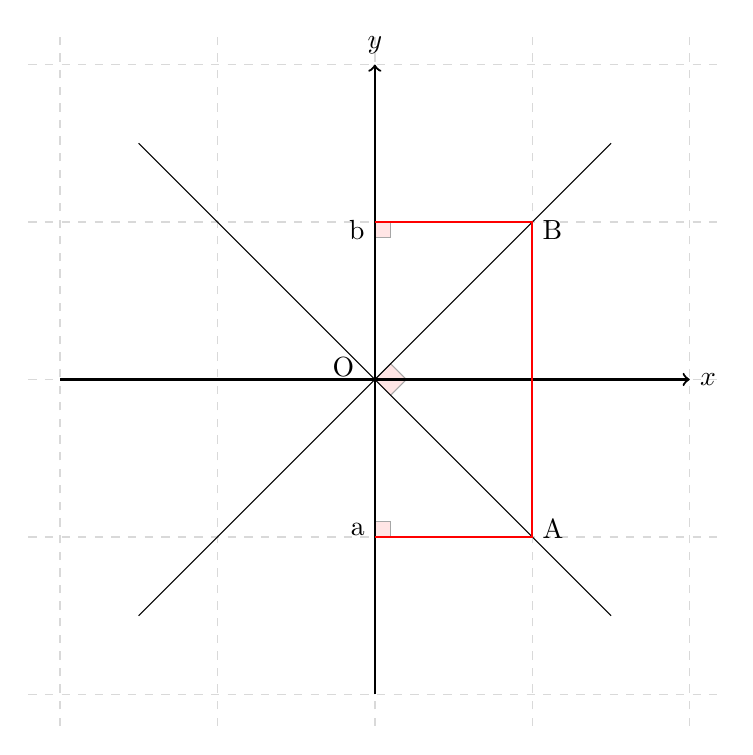
\begin{tikzpicture}[scale=2]
% define grid lines
\draw[help lines, color=gray!30, dashed, line width=0.5pt] (-2.2,-2.2) grid (2.2,2.2);

% mark right angles
\coordinate [label={[xshift=-0.4cm, yshift=-0.08cm]O}] (O) at (0,0);
\filldraw[fill=red!10,draw=gray!70] (1/10,-1/10) -- (2/10, 0) -- (1/10,1/10) -- (0,0);
\filldraw[fill=red!10,draw=gray!70] (0,1) -- (1/10, 1) -- (1/10,1-1/10) -- (0,1-1/10);
\filldraw[fill=red!10,draw=gray!70] (0,-1) -- (1/10, -1) -- (1/10,-1+1/10) -- (0,-1+1/10);

% define axis lines
\draw[->,thick] (-2,0)--(2,0) node[right]{$x$};
\draw[->,thick] (0,-2)--(0,2) node[above]{$y$};

% draw two orthogonal lines
\draw[black] (-1.5,-1.5) -- (1.5,1.5);
\draw[black] (1.5,-1.5) -- (-1.5,1.5);

% decorations
\draw[red,thick] (0,1) node[black,left,yshift={-0.1cm}] {b} -- (1,1) node[black,right,yshift={-0.1cm}] {B} -- (1,-1) node[black,right,yshift={0.1cm}] {A} -- (0,-1) node[black,left,yshift={0.1cm}] {a};

\end{tikzpicture} 

\end{document}
